\documentclass[12pt]{report}
\usepackage{graphicx}
\usepackage{algorithm}
\usepackage{algorithmic}

\usepackage{pdfcomment}
\newcommand{\note}[1]{\raisebox{0pt}[0pt][0pt]{\pdfcomment[open=true]{#1}}}

% [dme] reordered these document definitions - title, author, date -
% if they sit here, they can potentially use the macros you include
% from packages
\title{Avoiding the Dark Side}
\author{
        Leslie Chisholm \\
                Department of Computer Science\\
}
\date{\today}

\begin{document}
\maketitle

\begin{abstract}
This is the paper's abstract \ldots
\end{abstract}

\tableofcontents
\listoffigures\
\listofalgorithms
\chapter{Introduction}
This project focuses on how the sun shines on the city of Dunedin ...

\section{Goals}
The goals of this project were research and implement a sunlight projection model for the city of Dunedin. There are two parts; an interactive three-dimensional display to show point in time distribution of sunlight over Dunedin and a data aggregator to augment the display with computed measures of sunlight coverage over time ranges.

\section{Chapter outline}
In chapter x y will be presented...

\section{Background Information}
OpenGL is ... JOGL is ...
\note{Does `Background' normally sit in the introduction chapter? In a PhD thesis it would usually be chapter two. The problem with having it here is that the chapter outline comes after it. In most theses I've seen (these are not 480 project reports though) only the introduction text would come before the chapter outline.}


\chapter{Physical Data}
A digital elevation model of Dunedin and a mathematical model of the suns position\note{Not a model of the sun - a model of the sun's position. You need to be precise in this writing.} were gathered for this project...


\section{Elevation Data}
The elevation data was gathered from x and is encoded like y.


\subsection{Accuracy}
The accuracy of the elevation data was tested by doing x and y and these are the 
results...


\section{Sun}
The sun's\note{there aren't multiple `suns' for Earth!} current position in the sky can be accurately determined using these calculations: ...\\
and the time it rises and sets can be calculated by:...\\

Calculations of the sunset and sunrise times taken from \url{http://users.electromagnetic.net/bu/astro/sunrise-set.php} which is similar to the Wikipedia page on the sun. Calculations on that site were taken from here \url{http://www.astro.uu.nl/~strous/AA/en/reken/zonpositie.html}
\subsection{Calculating the Position of the Sun}
To calculate the position of the sun 


\subsection{Accuracy}
The accuracy of the sun was tested by doing x and y and these are the results...

\chapter{Viewer}
\begin{figure}[h]
\centering
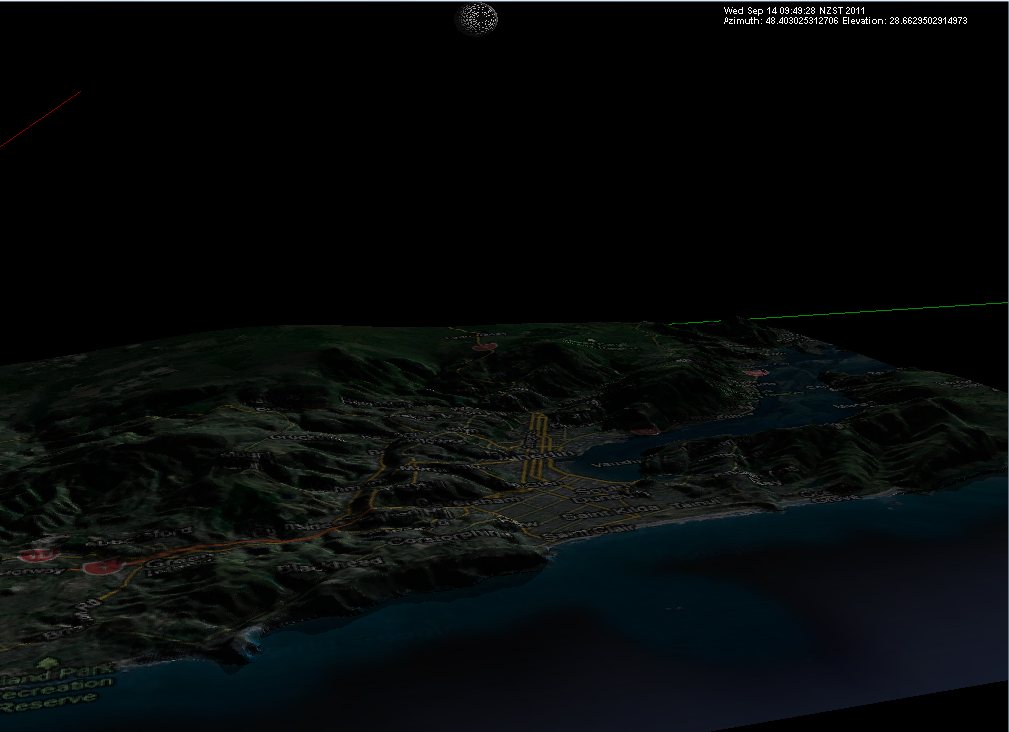
\includegraphics[scale=0.4]{viewer.png}
\caption{A screenshot of the viewer looking down at Dunedin}
\end{figure}\note{Good to see the screenshot! :-) Can the brightness/contrast be adjusted? It is very dark on my system.}
The viewer allows the user to view how the sun moves across the sky in a real-time 3D display...
\section{Drawing the elevation data}
The elevation data is drawn using OpenGL quads...
\section{Shadows}
Shadows are done on the graphics hardware using shadow maps...
\section{Usage}
The viewer can be run on any computer with a reasonably new graphics processor...
\subsection{Control}
The viewer can be controlled using the \texttt{w},\texttt{a},\texttt{s},and \texttt{d} keys to zoom in and out and mouse drags to rotate the screen...
\section{Future Work}
\chapter{Aggregator}
The aggregator is designed to calculate whether a portion of land is in shadow or not more accurately then using OpenGL methods such as shadow mapping...
\section{Algorithms Used}
A modified version of Cleary's algorithm was used to calculate whether a given block of land is in shadow or not... See algorithm~\ref{alg:shadow-calculation} for more information... \note{very nice! Always use named references though. I've fixed this instance.}

\begin{algorithm}[h]                      % enter the algorithm environment
\caption{Calculate whether a given point is in shadow or not}          % give the algorithm a caption
\label{alg:shadow-calculation}                           % and a label for \ref{} commands later in the document
\begin{algorithmic}                    % enter the algorithmic environment
\REQUIRE $n \geq 0 \vee x \neq 0$
\ENSURE $y = x^n$
\STATE $y \Leftarrow 1$
\IF{$n < 0$}
\STATE $X \Leftarrow 1 / x$
\STATE $N \Leftarrow -n$
\ELSE
\STATE $X \Leftarrow x$
\STATE $N \Leftarrow n$
\ENDIF
\WHILE{$N \neq 0$}
\IF{$N$ is even}
\STATE $X \Leftarrow X \times X$
\STATE $N \Leftarrow N / 2$
\ELSE[$N$ is odd]
\STATE $y \Leftarrow y \times X$
\STATE $N \Leftarrow N - 1$
\ENDIF
\ENDWHILE
\end{algorithmic}
\end{algorithm}

\section{Optimisations}
The aggregator can run faster by checking for shadows at the edges of an area of land. If there is no shadow present at any of the edges then it is safe to assume that none of the points within that region will be in shadow...\note{Good. Well expressed, too. Perhaps mention that there are more general forms of this optimisation strategy, but that there will be a cross-over point between the efficiency gained by not computing shadow rays against the extra effort in running the optimisation algorithm.}
\section{Data Gathered}
By runnning the aggregator for the whole year it was seen that suburb x managed to receive the highest amount of sun...
\section{Future work}
\chapter{Conclusion}
In the end the project was able to do x well and didn't do y as well as expected.
\bibliographystyle{abbrv}
\bibliography{480}

\end{document}
